% Dokumentklassen sættes til memoir.
% Manual: http://ctan.org/tex-archive/macros/latex/contrib/memoir/memman.pdf
\documentclass[a4paper,oneside,article,11pt]{memoir}

% Danske udtryk (fx figur og tabel) samt dansk orddeling og fonte med
% danske tegn. Hvis LaTeX brokker sig over æ, ø og å skal du udskifte
% "utf8" med "latin1" eller "applemac". 
\usepackage[utf8]{inputenc}
\usepackage[danish]{babel}
\usepackage{kpfonts}
\usepackage{float}

% Matematisk udtryk, fede symboler, theoremer og fancy ting (fx kædebrøker)
\usepackage{amsmath,amssymb}
\usepackage{bm}
\usepackage{amsthm}
\usepackage{mathtools}
\usepackage{gensymb}

\usepackage{multicol}

% Bruges til linkes i foodnoter og referencer.
\usepackage{hyperref}

% Kodelisting. Husk at læse manualen hvis du vil lave fancy ting.
% Manual: http://mirror.ctan.org/macros/latex/contrib/listings/listings.pdf
\usepackage{listings}

% Fancy ting med enheder og datatabeller. Læs manualen til pakken
% Manual: http://www.ctan.org/tex-archive/macros/latex/contrib/siunitx/siunitx.pdf
\usepackage{siunitx}

% Indsættelse af grafik.
\usepackage{graphicx}
\usepackage{braket}
\usepackage{caption}

% Reaktionsskemaer. Læs manualen for at se eksempler.
% Manual: http://www.ctan.org/tex-archive/macros/latex/contrib/mhchem/mhchem.pdf
\usepackage[margin=0.9in]{geometry}

\usepackage[version=3]{mhchem}
\usepackage{units}

\renewcommand{\baselinestretch}{1.1}




% Mine private funktioner og comandoer.
\newcommand{\dif}[1]{\frac{d}{d {#1}}}

\newcommand{\mylim}[2]{\lim\limits_{#1 \rightarrow #2}}

\newcommand{\myset}[2]{\left\{ #1 \mid #2 \right\} }

\newcommand{\funkt}[3]{#1 : #2 \rightarrow #3}

\newcommand{\funktt}[3]{#1 : #2 \rightarrow \mathbb{#3}}

\DeclareMathOperator{\Span}{Span}
\DeclareMathOperator{\sd}{sd}
\DeclareMathOperator{\Var}{Var}
\DeclareMathOperator{\Det}{Det}
\DeclareMathOperator{\Mat}{Mat}
\DeclareMathOperator{\Geo}{Geo}

\newenvironment{amatrix}[1]{%
  \left(\begin{array}{@{}*{#1}{c}|c@{}}
}{%
  \end{array}\right)
}

\parindent=0pt

\usepackage[framed,numbered,autolinebreaks,useliterate]{mcode}

\begin{document}

\title{Geometrisk Optik - Eksperimenter - Fysik Camp 2018}

\author{Christoffer H. og Jacob H.}

\maketitle
Dette er en øvelsesvejledningen til de forsøg, som I skal lave i Geometrisk Optik. Først er der dog en kort introduktion, til det der kaldes for ophobningsloven, som er en meget anvendt metode til at estimere usikkerheder i fysik.\\ 

\section*{Ophobningsloven}
Ophobningsloven er kort sagt en måde, hvorpå man kan bestemme usikkerheden af et udtryk, som selv er sammensat af størrelser med en usikkerhed. Et eksempel kunne f.eks. være, hvis man ville bestemme gennemsnitsfarten af en bil $v_{\text{av}}$, ved at måle både længden $L$ som bilen har kørt, og tiden $t$ som det tog bilen at køre stykket $L$. Da kan man bestemme gennemsnitsfarten som
\begin{align*}
v_{\text{av}} = \frac{L}{t} \, .
\end{align*}
Når man måler $L$ og $t$, vil der dog altid være en usikkerhed i disse målinger, $\sigma_L$ og $\sigma_t$, og der må derfor også være en usikkerhed i vores beregnede gennemsnitsfart $\sigma_{v_\text{av}}$. Spørgsmålet er så bare, hvad denne usikkerhed må være, og hvordan den afhænger af usikkerhederne $\sigma_L$ og $\sigma_t$? Svaret på disse spørgsmål er givet af ophobningsloven, der lyder således:\\ \\ \\

Hvis man skal beregne usikkerheden $\sigma_f$, for et udtryk $f$ som er sammensat af forskellige størrelser $a,b,c,\ldots$, så tænker man på ens udtryk som en funktion af disse, altså $f(a,b,c,\ldots)$, og usikkerheden vil da være givet ved:
\begin{align*}
\sigma_f = \sqrt{\left(\frac{\partial f}{\partial a}\right)^2 \cdot \sigma_a^2 + \left(\frac{\partial f}{\partial b}\right)^2 \cdot \sigma_b^2 + \left(\frac{\partial f}{\partial c}\right)^2 \cdot \sigma_c^2 + \cdots} \, \, \, ,
\end{align*}
hvor $\sigma_a,\sigma_b,\sigma_c,\ldots$ er usikkerhederne for hhv. $a,b,c,\ldots$. \\ \\ \\

For eksemplet med gennemsnitsfarten vil usikkerheden blive:
\begin{align*}
\sigma_{v_\text{av}}  = \sqrt{\frac{1}{t^2} \cdot \sigma_L^2 + \frac{L^2}{t^4} \cdot \sigma_t^2} \, \, .
\end{align*}
\newpage

\section*{Øvelsesvejledning}

\begin{figure}[h!]
	\centering
	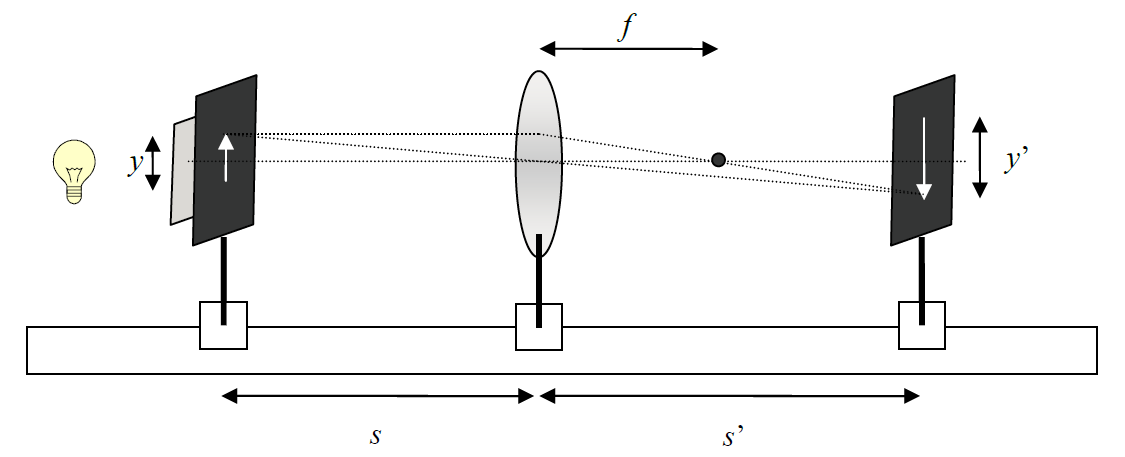
\includegraphics[scale=0.55]{linse-opstilling.png}
	\caption{Forsøgsopstilling med en enkelt linse.}
\end{figure}

\textbf{Første del}:
Undersøg, som beskrevet på side 111-112 i kompendiet, om billedafstanden $s'$ kommer tættere og tættere på fokallængden $f$, når man gør objektafstanden $s$ større og større. Altså at $s' \rightarrow f$, når $s \rightarrow \infty$. Vælg den linse som har den korteste fokallængde $f$ til denne del.\\

\textbf{Andel del}:
Tag et sæt af $15$ sammenhørende målinger af $s$ og $s'$, og indsæt dem i følgende skema. Her skal I også angive usikkerhederne for $s$ og $s'$ ved hver måling, som i selv skal estimere. 
\begin{table}[h!]
	\centering
	 \renewcommand*{\arraystretch}{1.3}
	\begin{tabular}{|l|l|l|l|}
		\hline
	$s \, \, \left[ \text{cm} \right]$	& $\sigma_s \, \, \left[ \text{cm} \right]$ & $s' \, \, \left[ \text{cm} \right]$ & $\sigma_{s'} \, \, \left[ \text{cm} \right]$  \\ \hline
		&  &  &  \\ \hline
		&  &  &  \\ \hline
		&  &  &  \\ \hline
		&  &  &  \\ \hline
		&  &  &  \\ \hline
		&  &  &  \\ \hline
		&  &  &  \\ \hline
		&  &  &  \\ \hline
		&  &  &  \\ \hline
		&  &  &  \\ \hline
		&  &  &  \\ \hline
		&  &  &  \\ \hline
		&  &  &  \\ \hline
		&  &  &  \\ \hline
		&  &  &  \\ \hline
	\end{tabular}
\end{table}

Beregn fokallængden $f$ som et gennemsnit af de første 5 målinger og bestem usikkerheden for dette gennemsnit $\sigma_f$. Gentag så dette, men nu hvor I tager alle 15 målinger med. Hvad sker der med usikkerheden $\sigma_f$, når man tager flere og flere målinger med? Hvordan kan dette forklares?\\

\textbf{Tredje del}:
Tag 3 af jeres målinger ($s$ og $s'$) fra før og bestem den tværgående forstørrelse
\begin{align*}
m = - \frac{s'}{s} \, .
\end{align*}
Tag målinger af $y$ (højden af objektet) og $y'$ (højden af billedet), for de 3 sæt af målinger I har valgt, og se om I får den samme forstørrelse vha. formlen:
\begin{align*}
m = \frac{y'}{y} \, .
\end{align*}

\textbf{Fjerde del}:
Brug den introducerede teori for linser i kompendiet, til at give et teoretisk bud på, hvad der sker, når man bruger to linser efter hinanden, hvor både objekt og billede for begge processer (brydning i hver linse) er placeret udenfor fokallængderne $f_1$ og $f_2$ for linserne.\\ 
Brug to linser til at lave et forstørrelsesglas, og indstil opstillingen så I får en forstørrelse $m$ på hhv. 1, 2 og 3. Stemmer længderne $s$ og $s'$ med det man ville forvente teoretisk?\\

\textbf{Ekstra del}:
Hvis I er hurtigt færdige med de andre dele, kan i kigge på denne. Her skal I prøve at bygge et teleskop vha. linserne I har til rådighed. Her skal i bruge definitionen af en vinkelforstørrelse, som er givet nedenunder, og kan få hjælp af figuren, der er placeret til sidst.\\

\emph{Vinkelforstørrelse}: I kompendiet blev den tværgående forstørrelse introduceret, men det er ikke den eneste måde at måle forstørrelsen. En anden måde er vinkelforstørrelsen. I stedet for at finde forholdet imellem højden af billedet og objektet, så finder man her forholdet mellem de vinkler, som objektet og billedet udspænder ift. den optiske akse (se evt. figuren nedenunder). Den er defineret som
\begin{align*}
m_\theta = \frac{\theta'}{\theta} \, \, \, \,  ,
\end{align*}
hvor $\theta$ refererer til objektet og $\theta'$ refererer til billedet.

\begin{figure}[h!]
	\centering
	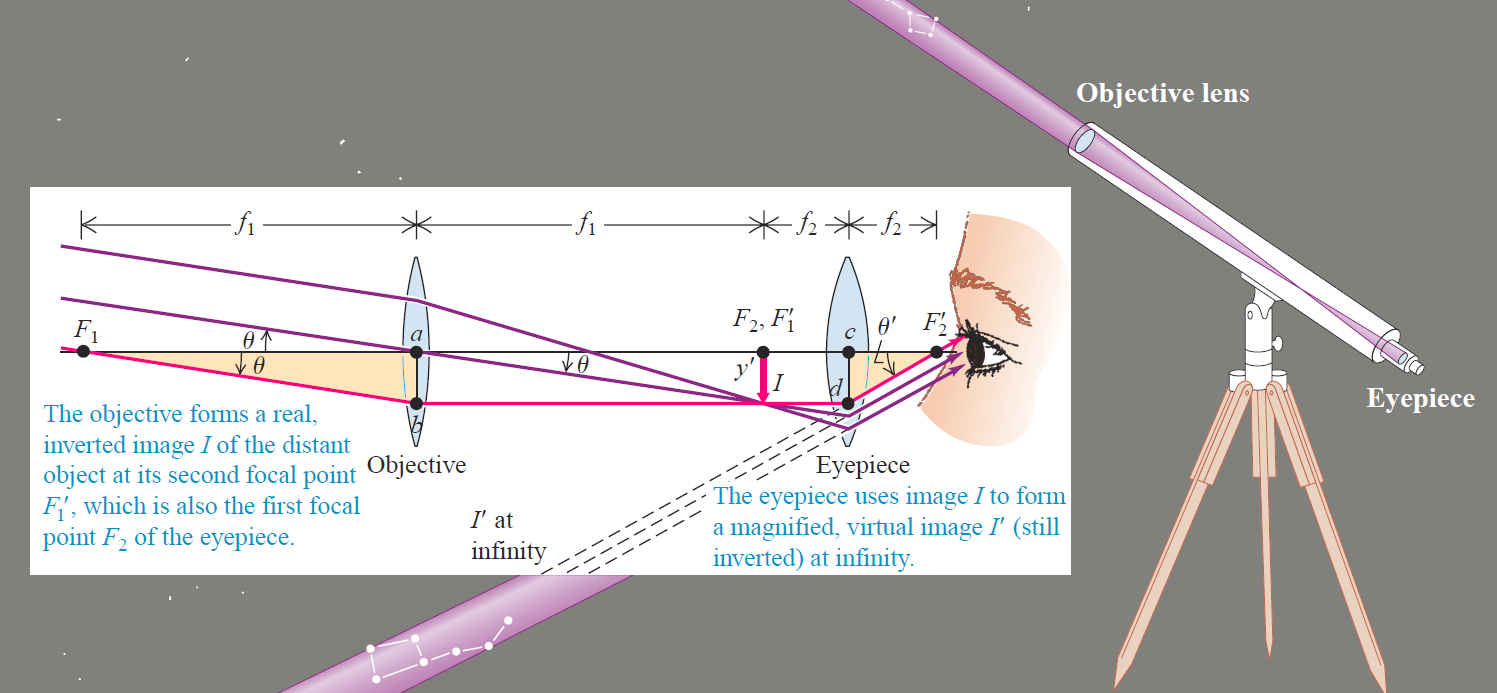
\includegraphics[scale=0.42]{teleskop-opstilling.png}
	\caption{Illustration af et teleskop.}
\end{figure}



\end{document}